\documentclass[11pt,letterpaper]{article}
\usepackage[margin=1in]{geometry}
\usepackage[T1]{fontenc}
\usepackage[utf8]{inputenc}
\usepackage{charter}
\usepackage{amsmath,amssymb}
\usepackage[dvipsnames]{xcolor}
\usepackage{graphicx}
\usepackage{booktabs}
\usepackage{longtable}
\usepackage{array}
\usepackage{pdflscape}
\usepackage{caption}
\usepackage{subcaption}
\usepackage{tikz}
\usetikzlibrary{arrows.meta,positioning,shadows.blur,fit,shapes.geometric,calc}
\usepackage{pgfplots}
\pgfplotsset{compat=1.18}
\usepackage{xurl}
\usepackage[colorlinks=true,linkcolor=MidnightBlue,urlcolor=MidnightBlue,citecolor=MidnightBlue]{hyperref}
\usepackage{bookmark}
\setlength{\parindent}{0pt}
\setlength{\parskip}{0.65em}
\captionsetup{font=small,labelfont=bf}
\newcommand{\filename}[1]{\nolinkurl{#1}}
\title{\bfseries Publication-Ready Evidence Report\\Blood-Vessel Segmentation in 3D Fluorescence Microscopy}
\author{Abdullah Al Bashit}
\date{Training job 6670898 and prediction job 6685455}
\begin{document}
\maketitle
\begin{abstract}
This report documents a transfer-learning Attention U-Net workflow for segmenting blood-vessel structures in noisy 3D fluorescence microscopy images. The study focuses on weak contrast, uneven focus, fragmented vessels, and limited annotations. The final model used a trainable pretrained ResNet34 encoder, attention-gated decoder skips, engineered image channels, and a Tversky-style loss. Across five held-out test images, the stitched-image Dice score was 0.9189 on average, and every held-out test image achieved Dice at least 0.90.
\end{abstract}
\tableofcontents
\clearpage
\section{Introduction}
Blood-vessel segmentation in fluorescence microscopy is difficult because the visual signal is not uniformly strong. Some vessels are bright and continuous, while others are faint, locally out of focus, or broken into short fragments. The goal of this work is therefore not only to train a segmentation model, but to understand how the model learns to recover weak vascular structure from noisy image evidence.
The report is written as an evidence package. It includes the dataset representation, model design, loss function, training protocol, validation attention progressions, final test comparisons, and failure-mode visualizations. Every validation and final-result figure identifies the original TIFF filename and split type so that the evidence can be audited image by image.
\section{Dataset and Input Representation}
The annotated dataset contained 25 image-mask pairs from day-7, day-14, and day-21 fluorescence microscopy acquisitions. The run used 20 images for training and cross-validation and 5 held-out images for the final test set. A separate prediction pass visualized 7 images: 2 train/validation pool images and all 5 held-out test images.
The model input at each pixel was a three-channel stack
\begin{equation}
\mathbf{x}(u,v) = \left[I(u,v),\, G(u,v),\, S(u,v)\right],
\end{equation}
where $I$ is the normalized grayscale fluorescence intensity, $G$ is an edge-strength channel, and $S$ is a local sharpness channel. These two engineered channels give the network explicit access to vessel boundaries and focus-related texture without requiring a much larger model to rediscover those cues from intensity alone.
The gradient magnitude channel was computed from Sobel derivatives:
\begin{equation}
G(u,v) = \sqrt{\left(\partial_x I(u,v)\right)^2 + \left(\partial_y I(u,v)\right)^2}.
\end{equation}
The sharpness channel used local variation in the Laplacian response:
\begin{equation}
S(u,v) = \operatorname{Var}_{\Omega(u,v)}\left(\nabla^2 I\right),
\end{equation}
where $\Omega(u,v)$ is a local window around the pixel. High values indicate locally crisp structures; low values indicate blurred or texture-poor regions.
\section{Preprocessing and Tiling}
The full images were processed as full-height horizontal strips. Each tile was 1300 pixels high and 1024 pixels wide, with a horizontal stride of 512 pixels. This design preserved long vertical context while keeping GPU memory use manageable. During stitched inference, overlapping tile predictions were blended with a Hann weighting map, optionally modulated by the sharpness channel so that locally reliable regions contributed more strongly to the final image-level prediction.
\section{Model Architecture}
The model was an Attention U-Net with a trainable pretrained ResNet34 encoder. Decoder skip connections were gated before fusion, allowing the model to suppress irrelevant encoder features while preserving vessel-like structures. A lightweight dilated refinement head produced the final logit map, which was converted to vessel probability by a sigmoid function.
\begin{figure}[htbp]
\centering
\resizebox{0.98\linewidth}{!}{%
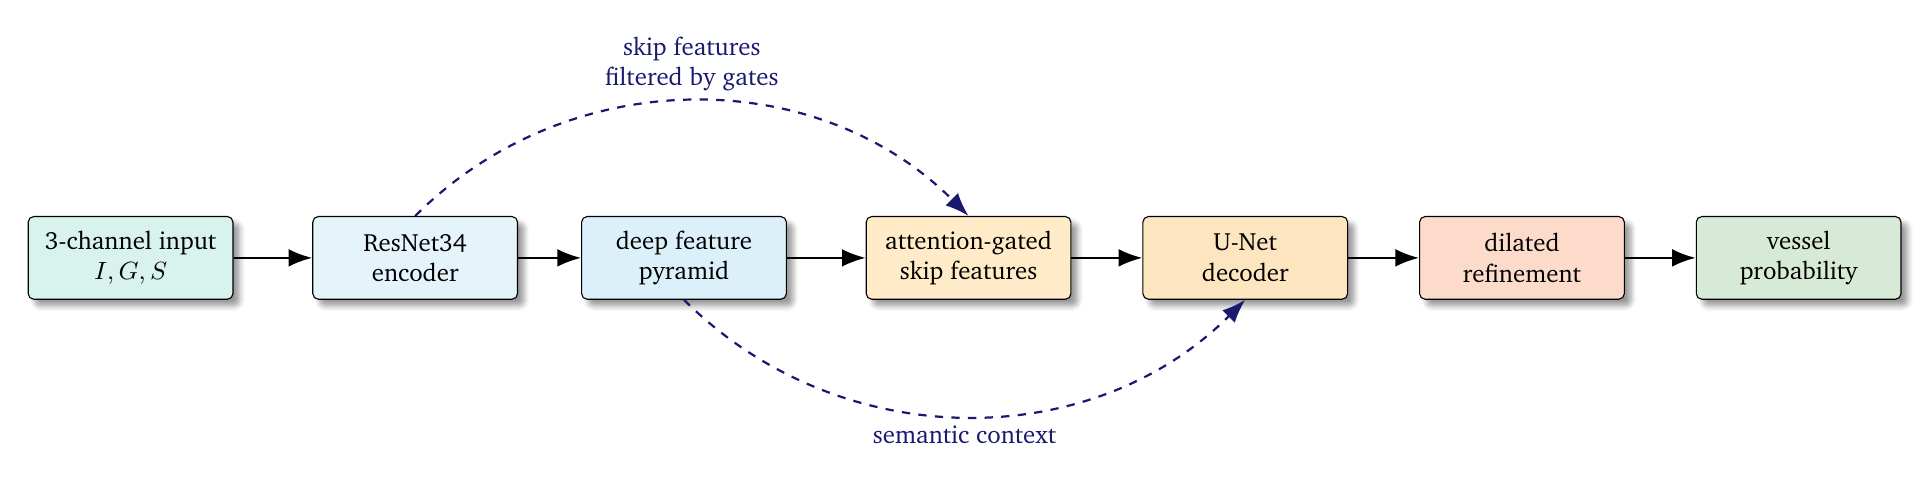
\begin{tikzpicture}[font=\small, box/.style={draw, rounded corners=2pt, minimum width=2.6cm, minimum height=1.05cm, align=center, fill=#1, blur shadow={shadow blur steps=5}}, arr/.style={-{Latex[length=3mm]}, thick}]
\node[box=BlueGreen!18] (input) {3-channel input\\$I, G, S$};
\node[box=SkyBlue!22, right=1.0cm of input] (enc1) {ResNet34\\encoder};
\node[box=SkyBlue!30, right=0.8cm of enc1] (enc2) {deep feature\\pyramid};
\node[box=Orange!22, right=1.0cm of enc2] (gate) {attention-gated\\skip features};
\node[box=YellowOrange!22, right=0.9cm of gate] (dec) {U-Net\\decoder};
\node[box=RedOrange!18, right=0.9cm of dec] (refine) {dilated\\refinement};
\node[box=ForestGreen!18, right=0.9cm of refine] (out) {vessel\\probability};
\draw[arr] (input) -- (enc1);
\draw[arr] (enc1) -- (enc2);
\draw[arr] (enc2) -- (gate);
\draw[arr] (gate) -- (dec);
\draw[arr] (dec) -- (refine);
\draw[arr] (refine) -- (out);
\draw[arr, dashed, MidnightBlue] (enc1.north) to[out=45,in=135] node[above, align=center] {skip features\\filtered by gates} (gate.north);
\draw[arr, dashed, MidnightBlue] (enc2.south) to[out=-45,in=-135] node[below, align=center] {semantic context} (dec.south);
\end{tikzpicture}%
}
\caption{Editable architecture schematic. The model receives intensity, gradient, and sharpness channels, processes them with a trainable pretrained ResNet34 encoder, filters skip features using attention gates, decodes vessel structure, refines the logits, and outputs a sigmoid vessel-probability map.}
\label{fig:architecture}
\end{figure}

\begin{landscape}
\begin{figure}[p]
\centering
\resizebox{0.99\linewidth}{!}{%
\begin{tikzpicture}[
font=\sffamily\scriptsize,
imagecard/.style={draw=white, line width=1.2pt, fill=white, rounded corners=2pt, inner sep=1.2pt, blur shadow={shadow blur steps=6, shadow opacity=0.22}},
mainarrow/.style={-{Latex[length=2.8mm,width=1.9mm]}, line width=1.05pt, draw=black!62},
skiparrow/.style={-{Latex[length=2.4mm,width=1.7mm]}, line width=0.92pt, draw=MidnightBlue!78},
gatearrow/.style={-{Latex[length=2.2mm,width=1.55mm]}, line width=0.88pt, draw=BurntOrange!82!black},
gate/.style={circle, minimum size=0.70cm, inner sep=1pt, draw=BurntOrange!72!black, fill=Orange!35, line width=0.72pt, font=\sffamily\tiny\bfseries, blur shadow={shadow blur steps=4, shadow opacity=0.12}},
head/.style={rounded corners=3pt, draw=ForestGreen!55!black, fill=ForestGreen!12, line width=0.75pt, minimum width=0.78cm, minimum height=0.72cm, align=center, blur shadow={shadow blur steps=4, shadow opacity=0.12}},
label/.style={font=\sffamily\scriptsize\bfseries, text=black!68, align=center},
tinylabel/.style={font=\sffamily\tiny, text=black!58, align=center}
]

\newcommand{\FeatureStack}[7]{%
  \begin{scope}[shift={#2}]
    \foreach \i/\shade in {0/50,1/40,2/31,3/23}{%
      \filldraw[draw=#5!72!black, fill=#5!\shade, line width=0.60pt, line join=round]
        ({0.13*\i},{0.09*\i}) -- ++(#3,0.26) -- ++(0,#4) -- ++(-#3,-0.26) -- cycle;
    }
    \coordinate (#1west) at (-0.03,{#4/2+0.12});
    \coordinate (#1east) at ({#3+0.50},{#4/2+0.38});
    \coordinate (#1north) at ({#3/2+0.24},{#4+0.33});
    \coordinate (#1south) at ({#3/2+0.24},-0.04);
    \ifstrempty{#6}{}{\node[tinylabel] at ({#3/2+0.24},-0.42) {#6};}
  \end{scope}
}

\node[font=\sffamily\small\bfseries, align=center] at (0,3.72) {Image-aware Attention U-Net};

% Upright input image stack
\node[imagecard] (img1) at (-6.80,1.86)
  {\includegraphics[width=1.30cm,height=1.62cm]{figures/report_images/prediction/originals_0_b01aa3ecab637aa430ca.png}};
\node[imagecard] (img2) at (-6.58,2.02)
  {\includegraphics[width=1.30cm,height=1.62cm]{figures/report_images/prediction/ch_grad_0_74cf9a898842fdc974eb.png}};
\node[imagecard] (img3) at (-6.36,2.18)
  {\includegraphics[width=1.30cm,height=1.62cm]{figures/report_images/prediction/ch_sharp_0_19a8b365298f5e350ecf.png}};
\node[tinylabel] at (-6.58,0.78) {3-channel input};
\node[tinylabel] at (-6.58,0.50) {image | gradient | sharpness};

% Encoder path
\FeatureStack{e0}{(-4.80,1.72)}{0.70}{1.28}{MidnightBlue}{}{}
\FeatureStack{e1}{(-4.10,0.50)}{0.58}{1.12}{MidnightBlue}{}{}
\FeatureStack{e2}{(-3.38,-0.70)}{0.48}{0.96}{MidnightBlue}{}{}
\FeatureStack{e3}{(-2.70,-1.90)}{0.38}{0.82}{MidnightBlue}{}{}
\FeatureStack{bn}{(-0.45,-2.86)}{0.42}{0.70}{Purple}{bottleneck}{}

% Decoder path
\FeatureStack{d3}{(2.10,-1.90)}{0.38}{0.82}{BurntOrange}{}{}
\FeatureStack{d2}{(2.78,-0.70)}{0.48}{0.96}{BurntOrange}{}{}
\FeatureStack{d1}{(3.48,0.50)}{0.58}{1.12}{BurntOrange}{}{}
\FeatureStack{d0}{(4.18,1.72)}{0.70}{1.28}{BurntOrange}{}{}
\node[head] (head) at (5.67,2.42) {$1{\times}1$};
\node[tinylabel, below=0.12cm of head] {sigmoid};

% Upright output image stack
\node[imagecard] (out1) at (7.00,1.92)
  {\includegraphics[width=1.30cm,height=1.62cm]{figures/report_images/prediction/prediction_0_908ccf4cb56e55558686.png}};
\node[imagecard] (out2) at (7.22,2.08)
  {\includegraphics[width=1.30cm,height=1.62cm]{figures/report_images/prediction/combined_0_f919a479b44de7fb61b4.png}};
\node[tinylabel] at (7.12,0.78) {output stack};
\node[tinylabel] at (7.12,0.50) {probability | TP/FP/FN};

% Main U-shaped flow
\draw[mainarrow] (img3.east) -- (e0west);
\draw[mainarrow] (e0south) -- (e1north);
\draw[mainarrow] (e1south) -- (e2north);
\draw[mainarrow] (e2south) -- (e3north);
\draw[mainarrow] (e3east) -- (bnwest);
\draw[mainarrow] (bneast) -- (d3west);
\draw[mainarrow] (d3north) -- (d2south);
\draw[mainarrow] (d2north) -- (d1south);
\draw[mainarrow] (d1north) -- (d0south);
\draw[mainarrow] (d0east) -- (head.west);
\draw[mainarrow] (head.east) -- (out1.west);

% Attention-gated skip connections
\node[gate] (a0) at (0.00,2.36) {attn0};
\node[gate] (a1) at (0.00,1.20) {attn1};
\node[gate] (a2) at (0.00,0.00) {attn2};
\node[gate] (a3) at (0.00,-1.20) {attn3};

\draw[skiparrow] (e0east) -- (a0.west);
\draw[gatearrow] (a0.east) -- (d0west);
\draw[skiparrow] (e1east) -- (a1.west);
\draw[gatearrow] (a1.east) -- (d1west);
\draw[skiparrow] (e2east) -- (a2.west);
\draw[gatearrow] (a2.east) -- (d2west);
\draw[skiparrow] (e3east) -- (a3.west);
\draw[gatearrow] (a3.east) -- (d3west);

\end{tikzpicture}%
}
\caption{U-shaped stacked implementation schematic for the Attention U-Net. Real report panels from \filename{16\_20250731\_Plate1\_A1\_D14\_MAX\_Crop.tif} are kept upright and stacked at the input and output. Editable TikZ feature stacks show the ResNet34 encoder, bottleneck, attention-gated skip connections, decoder, and sigmoid output head.}
\label{fig:architecture-detail}
\end{figure}
\end{landscape}

Figure~\ref{fig:architecture-detail} labels the gated skip modules as Attn0--Attn3. Attn1--Attn3 correspond to the attention panels shown later; Attn0 is the finest-scale stem gate. Each gated skip is added to the decoder state before the next upsampling step.
The attention gate can be written as
\begin{equation}
\alpha_l = \sigma\left(\psi_l^\top \operatorname{ReLU}(W_x x_l + W_g g_l + b_l)\right), \qquad \tilde{x}_l = \alpha_l \odot x_l,
\end{equation}
where $x_l$ is the encoder skip feature, $g_l$ is the decoder gating signal, and $\tilde{x}_l$ is the filtered skip feature passed to the decoder.
\section{Loss Function and Optimization}
The final run used a Tversky-style vessel loss. For predicted probability $p_i$ and binary mask $y_i$, the soft true-positive, false-positive, and false-negative terms are
\begin{equation}
TP=\sum_i p_i y_i,\qquad FP=\sum_i p_i(1-y_i),\qquad FN=\sum_i (1-p_i)y_i.
\end{equation}
The loss was
\begin{equation}
\mathcal{L}_{\mathrm{Tv}} = 1 - \frac{TP+\epsilon}{TP+\alpha FP+\beta FN+\epsilon},
\end{equation}
with the configured final run using $\beta=0.5$ and the Tversky term as the active segmentation loss. The model probability was $p_i=\sigma(z_i)$, where $z_i$ is the output logit.
\section{Training Protocol}
Training ran on the Explorer HPC cluster as job 6670898 using an NVIDIA A100-SXM4-40GB GPU, CUDA 12.1, and PyTorch 2.5.1+cu121. The optimizer was AdamW with learning rate $10^{-4}$ and weight decay $10^{-4}$, followed by cosine annealing to $10^{-6}$. The maximum training budget was 100 epochs, batch size was 12, and early stopping was applied independently within each fold with patience 30. Automatic mixed precision and gradient clipping were used during CUDA training. The final prediction pass ran as job 6685455 on a Tesla V100-SXM2-32GB GPU.
\begin{table}[htbp]
\centering
\caption{Training and inference configuration.}
\begin{tabular}{ll}
\toprule
Item & Value \\
\midrule
Training job & 6670898 on Explorer HPC \\
Training GPU & NVIDIA A100-SXM4-40GB \\
Prediction job & 6685455 on Explorer HPC \\
Prediction GPU & Tesla V100-SXM2-32GB \\
Software & CUDA 12.1, PyTorch 2.5.1+cu121 \\
Cross-validation & 5 folds \\
Batch size & 12 \\
Optimizer & AdamW, learning rate $10^{-4}$, weight decay $10^{-4}$ \\
Scheduler & Cosine annealing to $10^{-6}$ \\
Early stopping & patience 30, maximum 100 epochs \\
\bottomrule
\end{tabular}
\label{tab:training-info}
\end{table}
\section{Results}
\begin{table}[htbp]
\centering
\caption{Five-fold validation summary. Fold 1 was selected for final held-out evaluation.}
\begin{tabular}{cccc}
\toprule
Fold & Best epoch & Validation loss & Status \\
\midrule
1 & 48 & 0.0568 & selected \\
2 & 33 & 0.0713 &  \\
3 & 37 & 0.0627 &  \\
4 & 23 & 0.0624 &  \\
5 & 22 & 0.0721 &  \\
\bottomrule
\end{tabular}
\label{tab:fold-results}
\end{table}
\begin{table}[htbp]
\centering
\caption{Final held-out test-set performance.}
\begin{tabular}{lc}
\toprule
Metric & Value \\
\midrule
Cross-validation mean $\pm$ std & $0.0651 \pm 0.0058$ \\
Test loss & 0.0662 \\
Tile-level test Dice & 0.9158 \\
Mean stitched-image Dice & 0.9189 \\
Stitched-image Dice std & 0.0164 \\
95\% confidence interval & [0.8962, 0.9417] \\
Held-out test images with Dice $\ge 0.90$ & 5/5 \\
\bottomrule
\end{tabular}
\label{tab:test-results}
\end{table}
\begin{figure}[htbp]
\centering
\begin{tikzpicture}
\begin{axis}[width=0.92\linewidth,height=7cm,xlabel={Epoch},ylabel={Validation loss},legend pos=north east,grid=both]
\addplot[MidnightBlue, thick] table[x=epoch,y=val_loss]{figures/plots/fold1_curves.dat};
\addlegendentry{Fold 1}
\addplot[RedOrange, thick] table[x=epoch,y=val_loss]{figures/plots/fold2_curves.dat};
\addlegendentry{Fold 2}
\addplot[ForestGreen, thick] table[x=epoch,y=val_loss]{figures/plots/fold3_curves.dat};
\addlegendentry{Fold 3}
\addplot[Purple, thick] table[x=epoch,y=val_loss]{figures/plots/fold4_curves.dat};
\addlegendentry{Fold 4}
\addplot[TealBlue, thick] table[x=epoch,y=val_loss]{figures/plots/fold5_curves.dat};
\addlegendentry{Fold 5}
\end{axis}
\end{tikzpicture}
\caption{Editable PGFPlots validation-loss curves parsed from \nolinkurl{train_6670898.out}. Fold 1 achieved the lowest validation loss and was used for final held-out inference.}
\label{fig:val-curves}
\end{figure}
\section{Attention Progression During Training}
The following validation figures show how the model's vessel probability and attention gates changed during training. Each figure explicitly names the validation TIFF, fold, and epochs shown. The attention overlays are not final test evidence; they are fold-level validation snapshots used to inspect learning behavior.
\subsection{Fold 1 Validation Image}
\nolinkurl{13_20250724_Plate1_C3_D7_MAX_Crop.tif} is the fold 1 validation image. The progression shows the model moving from broad vessel-like responses toward cleaner vessel masks as the validation loss stabilizes. The three attention-gate rows expose which decoder stages are emphasizing high-confidence vessel regions and which stages still respond to ambiguous background structure.
\begin{landscape}
\begin{figure}[p]
\centering
\scriptsize
\setlength{\tabcolsep}{2pt}
\renewcommand{\arraystretch}{0.9}
\textbf{Fold 1 validation image: \nolinkurl{13_20250724_Plate1_C3_D7_MAX_Crop.tif}}\\[0.4em]
\begin{tabular}{lcccc}
 & Input & Gradient magnitude & Sharpness map & Ground truth \\
Reference & \includegraphics[height=0.105\linewidth]{figures/report_images/training/fold1/input_image_10_18354afca2e57607e2eb.png} & \includegraphics[height=0.105\linewidth]{figures/report_images/training/fold1/ch_grad_10_3eb077088a5f961fc783.png} & \includegraphics[height=0.105\linewidth]{figures/report_images/training/fold1/ch_sharp_10_5e3770845454a63270a2.png} & \includegraphics[height=0.105\linewidth]{figures/report_images/training/fold1/gt_mask_10_95ae520d05c0cf04fd34.png} \\
\end{tabular}
\vspace{0.5em}
\begin{tabular}{lccccccc}
 & Epoch 10 & Epoch 20 & Epoch 30 & Epoch 40 & Epoch 50 & Epoch 60 & Epoch 70 \\
Probability & \includegraphics[height=0.088\linewidth]{figures/report_images/training/fold1/pred_prob_10_cd03861fe91aa6fe40d9.png} & \includegraphics[height=0.088\linewidth]{figures/report_images/training/fold1/pred_prob_21_11b4f7b552bccb04193a.png} & \includegraphics[height=0.088\linewidth]{figures/report_images/training/fold1/pred_prob_32_e7fc96357be76d8f5527.png} & \includegraphics[height=0.088\linewidth]{figures/report_images/training/fold1/pred_prob_43_dbc3b66d9f8eeb51d528.png} & \includegraphics[height=0.088\linewidth]{figures/report_images/training/fold1/pred_prob_54_b4501f1a3cecc1f2371b.png} & \includegraphics[height=0.088\linewidth]{figures/report_images/training/fold1/pred_prob_65_ff3421550fdeac914d94.png} & \includegraphics[height=0.088\linewidth]{figures/report_images/training/fold1/pred_prob_76_1eea62d3057858b9c249.png} \\
Binary mask & \includegraphics[height=0.088\linewidth]{figures/report_images/training/fold1/pred_binary_10_3b90580940e0c5fc10f1.png} & \includegraphics[height=0.088\linewidth]{figures/report_images/training/fold1/pred_binary_21_89ff2df30d3062d6c38e.png} & \includegraphics[height=0.088\linewidth]{figures/report_images/training/fold1/pred_binary_32_c31e9cd653952d2b9a79.png} & \includegraphics[height=0.088\linewidth]{figures/report_images/training/fold1/pred_binary_43_85ce19c9c4c2730709fe.png} & \includegraphics[height=0.088\linewidth]{figures/report_images/training/fold1/pred_binary_54_3dba20d3db1f340aafca.png} & \includegraphics[height=0.088\linewidth]{figures/report_images/training/fold1/pred_binary_65_e09805658766a2c4fa0b.png} & \includegraphics[height=0.088\linewidth]{figures/report_images/training/fold1/pred_binary_76_3d5779563ba12cb69a96.png} \\
Attention gate 1 & \includegraphics[height=0.088\linewidth]{figures/report_images/training/fold1/attn1_overlay_10_a17898c946c7d1e94797.png} & \includegraphics[height=0.088\linewidth]{figures/report_images/training/fold1/attn1_overlay_21_01beaa81a63181d3aa4d.png} & \includegraphics[height=0.088\linewidth]{figures/report_images/training/fold1/attn1_overlay_32_47f1df20220e54f85373.png} & \includegraphics[height=0.088\linewidth]{figures/report_images/training/fold1/attn1_overlay_43_f37d44237c8f026690d3.png} & \includegraphics[height=0.088\linewidth]{figures/report_images/training/fold1/attn1_overlay_54_088f2964a5bbce6faf34.png} & \includegraphics[height=0.088\linewidth]{figures/report_images/training/fold1/attn1_overlay_65_955832579e7c23e1b6d6.png} & \includegraphics[height=0.088\linewidth]{figures/report_images/training/fold1/attn1_overlay_76_33b045407cbbd7c0d313.png} \\
Attention gate 2 & \includegraphics[height=0.088\linewidth]{figures/report_images/training/fold1/attn2_overlay_10_99f35c88c0de54e5b496.png} & \includegraphics[height=0.088\linewidth]{figures/report_images/training/fold1/attn2_overlay_21_baf06e9ace6541436c0d.png} & \includegraphics[height=0.088\linewidth]{figures/report_images/training/fold1/attn2_overlay_32_304afdba2ccdcfae5608.png} & \includegraphics[height=0.088\linewidth]{figures/report_images/training/fold1/attn2_overlay_43_3cbc9fa261d07b70e988.png} & \includegraphics[height=0.088\linewidth]{figures/report_images/training/fold1/attn2_overlay_54_6b9290514b2f57fdd80c.png} & \includegraphics[height=0.088\linewidth]{figures/report_images/training/fold1/attn2_overlay_65_178eb564eae813b31457.png} & \includegraphics[height=0.088\linewidth]{figures/report_images/training/fold1/attn2_overlay_76_aae107db7a81438535cf.png} \\
Attention gate 3 & \includegraphics[height=0.088\linewidth]{figures/report_images/training/fold1/attn3_overlay_10_7998c7be5efbd6ea905a.png} & \includegraphics[height=0.088\linewidth]{figures/report_images/training/fold1/attn3_overlay_21_a52937117ef0c1f8c565.png} & \includegraphics[height=0.088\linewidth]{figures/report_images/training/fold1/attn3_overlay_32_4a0a92bb5cd90330684a.png} & \includegraphics[height=0.088\linewidth]{figures/report_images/training/fold1/attn3_overlay_43_26ddf314365aff9686ae.png} & \includegraphics[height=0.088\linewidth]{figures/report_images/training/fold1/attn3_overlay_54_8b50e45204931fcf7eda.png} & \includegraphics[height=0.088\linewidth]{figures/report_images/training/fold1/attn3_overlay_65_a45d3d21a16d19543a14.png} & \includegraphics[height=0.088\linewidth]{figures/report_images/training/fold1/attn3_overlay_76_6654d1b5b6e8fc4eeb69.png} \\
\end{tabular}
\caption{Step-by-step training progress for validation image \nolinkurl{13_20250724_Plate1_C3_D7_MAX_Crop.tif} in fold 1. The split type is validation and the epochs shown are 10, 20, 30, 40, 50, 60, 70. The top reference row shows the input image, engineered gradient channel, sharpness channel, and ground-truth vessel mask. The epoch rows show probability maps, thresholded binary masks, and attention overlays from gates 1--3. Hotter attention colors indicate regions receiving stronger gating weight during decoding.}
\label{fig:fold1-progress}
\end{figure}
\end{landscape}

\begin{landscape}
\begin{figure}[p]
\centering
\scriptsize
\setlength{\tabcolsep}{2pt}
\begin{tabular}{lccccccc}
 & Epoch 10 & Epoch 20 & Epoch 30 & Epoch 40 & Epoch 50 & Epoch 60 & Epoch 70 \\
Gate 1 & \includegraphics[height=0.14\linewidth]{figures/report_images/training/fold1/attn1_overlay_10_a17898c946c7d1e94797.png} & \includegraphics[height=0.14\linewidth]{figures/report_images/training/fold1/attn1_overlay_21_01beaa81a63181d3aa4d.png} & \includegraphics[height=0.14\linewidth]{figures/report_images/training/fold1/attn1_overlay_32_47f1df20220e54f85373.png} & \includegraphics[height=0.14\linewidth]{figures/report_images/training/fold1/attn1_overlay_43_f37d44237c8f026690d3.png} & \includegraphics[height=0.14\linewidth]{figures/report_images/training/fold1/attn1_overlay_54_088f2964a5bbce6faf34.png} & \includegraphics[height=0.14\linewidth]{figures/report_images/training/fold1/attn1_overlay_65_955832579e7c23e1b6d6.png} & \includegraphics[height=0.14\linewidth]{figures/report_images/training/fold1/attn1_overlay_76_33b045407cbbd7c0d313.png} \\
Gate 2 & \includegraphics[height=0.14\linewidth]{figures/report_images/training/fold1/attn2_overlay_10_99f35c88c0de54e5b496.png} & \includegraphics[height=0.14\linewidth]{figures/report_images/training/fold1/attn2_overlay_21_baf06e9ace6541436c0d.png} & \includegraphics[height=0.14\linewidth]{figures/report_images/training/fold1/attn2_overlay_32_304afdba2ccdcfae5608.png} & \includegraphics[height=0.14\linewidth]{figures/report_images/training/fold1/attn2_overlay_43_3cbc9fa261d07b70e988.png} & \includegraphics[height=0.14\linewidth]{figures/report_images/training/fold1/attn2_overlay_54_6b9290514b2f57fdd80c.png} & \includegraphics[height=0.14\linewidth]{figures/report_images/training/fold1/attn2_overlay_65_178eb564eae813b31457.png} & \includegraphics[height=0.14\linewidth]{figures/report_images/training/fold1/attn2_overlay_76_aae107db7a81438535cf.png} \\
Gate 3 & \includegraphics[height=0.14\linewidth]{figures/report_images/training/fold1/attn3_overlay_10_7998c7be5efbd6ea905a.png} & \includegraphics[height=0.14\linewidth]{figures/report_images/training/fold1/attn3_overlay_21_a52937117ef0c1f8c565.png} & \includegraphics[height=0.14\linewidth]{figures/report_images/training/fold1/attn3_overlay_32_4a0a92bb5cd90330684a.png} & \includegraphics[height=0.14\linewidth]{figures/report_images/training/fold1/attn3_overlay_43_26ddf314365aff9686ae.png} & \includegraphics[height=0.14\linewidth]{figures/report_images/training/fold1/attn3_overlay_54_8b50e45204931fcf7eda.png} & \includegraphics[height=0.14\linewidth]{figures/report_images/training/fold1/attn3_overlay_65_a45d3d21a16d19543a14.png} & \includegraphics[height=0.14\linewidth]{figures/report_images/training/fold1/attn3_overlay_76_6654d1b5b6e8fc4eeb69.png} \\
\end{tabular}
\caption{Attention-only view for validation image \nolinkurl{13_20250724_Plate1_C3_D7_MAX_Crop.tif} in fold 1. The split type is validation and columns are epochs 10, 20, 30, 40, 50, 60, 70. Rows correspond to the three attention gates in the decoder, allowing coarse-to-fine changes in feature selection to be inspected without the probability-mask rows.}
\label{fig:fold1-attention}
\end{figure}
\end{landscape}

\subsection{Fold 2 Validation Image}
\nolinkurl{42_20250807_Plate1_C2_D21_MAX_Crop.tif} is the fold 2 validation image. The progression shows the model moving from broad vessel-like responses toward cleaner vessel masks as the validation loss stabilizes. The three attention-gate rows expose which decoder stages are emphasizing high-confidence vessel regions and which stages still respond to ambiguous background structure.
\begin{landscape}
\begin{figure}[p]
\centering
\scriptsize
\setlength{\tabcolsep}{2pt}
\renewcommand{\arraystretch}{0.9}
\textbf{Fold 2 validation image: \nolinkurl{42_20250807_Plate1_C2_D21_MAX_Crop.tif}}\\[0.4em]
\begin{tabular}{lcccc}
 & Input & Gradient magnitude & Sharpness map & Ground truth \\
Reference & \includegraphics[height=0.105\linewidth]{figures/report_images/training/fold2/input_image_96_74c96aeb10d1306503e2.png} & \includegraphics[height=0.105\linewidth]{figures/report_images/training/fold2/ch_grad_96_0ef189866f989d8bda31.png} & \includegraphics[height=0.105\linewidth]{figures/report_images/training/fold2/ch_sharp_96_d183a452d0f4b4de4d87.png} & \includegraphics[height=0.105\linewidth]{figures/report_images/training/fold2/gt_mask_96_2aafdc018a8f30299a82.png} \\
\end{tabular}
\vspace{0.5em}
\begin{tabular}{lcccccc}
 & Epoch 10 & Epoch 20 & Epoch 30 & Epoch 40 & Epoch 50 & Epoch 60 \\
Probability & \includegraphics[height=0.088\linewidth]{figures/report_images/training/fold2/pred_prob_96_b51ebc2bacc7eefe5e2b.png} & \includegraphics[height=0.088\linewidth]{figures/report_images/training/fold2/pred_prob_107_c2e5f1934f4aa44f9d59.png} & \includegraphics[height=0.088\linewidth]{figures/report_images/training/fold2/pred_prob_118_03d337b3be63284b8262.png} & \includegraphics[height=0.088\linewidth]{figures/report_images/training/fold2/pred_prob_129_fa0df6eff694e90b6a3e.png} & \includegraphics[height=0.088\linewidth]{figures/report_images/training/fold2/pred_prob_140_01e644ce0bd8e187baa8.png} & \includegraphics[height=0.088\linewidth]{figures/report_images/training/fold2/pred_prob_151_f777cf68773ff28ee724.png} \\
Binary mask & \includegraphics[height=0.088\linewidth]{figures/report_images/training/fold2/pred_binary_96_06dbfb8a5713b196ccf2.png} & \includegraphics[height=0.088\linewidth]{figures/report_images/training/fold2/pred_binary_107_a4e4de45065c1740fca4.png} & \includegraphics[height=0.088\linewidth]{figures/report_images/training/fold2/pred_binary_118_2cf314de932313cce17a.png} & \includegraphics[height=0.088\linewidth]{figures/report_images/training/fold2/pred_binary_129_33574dbfa23a0393c464.png} & \includegraphics[height=0.088\linewidth]{figures/report_images/training/fold2/pred_binary_140_23d950fc7c24a02af624.png} & \includegraphics[height=0.088\linewidth]{figures/report_images/training/fold2/pred_binary_151_e62169b0ead950513ac8.png} \\
Attention gate 1 & \includegraphics[height=0.088\linewidth]{figures/report_images/training/fold2/attn1_overlay_96_92b5c5683dd338418d6b.png} & \includegraphics[height=0.088\linewidth]{figures/report_images/training/fold2/attn1_overlay_107_1b16ef67fceaecb6104c.png} & \includegraphics[height=0.088\linewidth]{figures/report_images/training/fold2/attn1_overlay_118_bd6d10699df7ade1aab7.png} & \includegraphics[height=0.088\linewidth]{figures/report_images/training/fold2/attn1_overlay_129_67a37354c06d76e2f63b.png} & \includegraphics[height=0.088\linewidth]{figures/report_images/training/fold2/attn1_overlay_140_532b41f38fcc155db3e1.png} & \includegraphics[height=0.088\linewidth]{figures/report_images/training/fold2/attn1_overlay_151_b8590bcde7fb586179c6.png} \\
Attention gate 2 & \includegraphics[height=0.088\linewidth]{figures/report_images/training/fold2/attn2_overlay_96_f16492dcf4da8591e28c.png} & \includegraphics[height=0.088\linewidth]{figures/report_images/training/fold2/attn2_overlay_107_d0214e7dea4a6505399b.png} & \includegraphics[height=0.088\linewidth]{figures/report_images/training/fold2/attn2_overlay_118_17e348512e6768d35203.png} & \includegraphics[height=0.088\linewidth]{figures/report_images/training/fold2/attn2_overlay_129_e78e3a3b2413174d5acb.png} & \includegraphics[height=0.088\linewidth]{figures/report_images/training/fold2/attn2_overlay_140_83c21b4db04eb44dc146.png} & \includegraphics[height=0.088\linewidth]{figures/report_images/training/fold2/attn2_overlay_151_f682cab8314890760e10.png} \\
Attention gate 3 & \includegraphics[height=0.088\linewidth]{figures/report_images/training/fold2/attn3_overlay_96_49018201b2c023c1b008.png} & \includegraphics[height=0.088\linewidth]{figures/report_images/training/fold2/attn3_overlay_107_554a640b3b0fd104e498.png} & \includegraphics[height=0.088\linewidth]{figures/report_images/training/fold2/attn3_overlay_118_17a23ae8799b3ca9755d.png} & \includegraphics[height=0.088\linewidth]{figures/report_images/training/fold2/attn3_overlay_129_2717153ed09c2d85c0c9.png} & \includegraphics[height=0.088\linewidth]{figures/report_images/training/fold2/attn3_overlay_140_f859b9cd542c157c5589.png} & \includegraphics[height=0.088\linewidth]{figures/report_images/training/fold2/attn3_overlay_151_3143a4454a9b12c6b363.png} \\
\end{tabular}
\caption{Step-by-step training progress for validation image \nolinkurl{42_20250807_Plate1_C2_D21_MAX_Crop.tif} in fold 2. The split type is validation and the epochs shown are 10, 20, 30, 40, 50, 60. The top reference row shows the input image, engineered gradient channel, sharpness channel, and ground-truth vessel mask. The epoch rows show probability maps, thresholded binary masks, and attention overlays from gates 1--3. Hotter attention colors indicate regions receiving stronger gating weight during decoding.}
\label{fig:fold2-progress}
\end{figure}
\end{landscape}

\begin{landscape}
\begin{figure}[p]
\centering
\scriptsize
\setlength{\tabcolsep}{2pt}
\begin{tabular}{lcccccc}
 & Epoch 10 & Epoch 20 & Epoch 30 & Epoch 40 & Epoch 50 & Epoch 60 \\
Gate 1 & \includegraphics[height=0.14\linewidth]{figures/report_images/training/fold2/attn1_overlay_96_92b5c5683dd338418d6b.png} & \includegraphics[height=0.14\linewidth]{figures/report_images/training/fold2/attn1_overlay_107_1b16ef67fceaecb6104c.png} & \includegraphics[height=0.14\linewidth]{figures/report_images/training/fold2/attn1_overlay_118_bd6d10699df7ade1aab7.png} & \includegraphics[height=0.14\linewidth]{figures/report_images/training/fold2/attn1_overlay_129_67a37354c06d76e2f63b.png} & \includegraphics[height=0.14\linewidth]{figures/report_images/training/fold2/attn1_overlay_140_532b41f38fcc155db3e1.png} & \includegraphics[height=0.14\linewidth]{figures/report_images/training/fold2/attn1_overlay_151_b8590bcde7fb586179c6.png} \\
Gate 2 & \includegraphics[height=0.14\linewidth]{figures/report_images/training/fold2/attn2_overlay_96_f16492dcf4da8591e28c.png} & \includegraphics[height=0.14\linewidth]{figures/report_images/training/fold2/attn2_overlay_107_d0214e7dea4a6505399b.png} & \includegraphics[height=0.14\linewidth]{figures/report_images/training/fold2/attn2_overlay_118_17e348512e6768d35203.png} & \includegraphics[height=0.14\linewidth]{figures/report_images/training/fold2/attn2_overlay_129_e78e3a3b2413174d5acb.png} & \includegraphics[height=0.14\linewidth]{figures/report_images/training/fold2/attn2_overlay_140_83c21b4db04eb44dc146.png} & \includegraphics[height=0.14\linewidth]{figures/report_images/training/fold2/attn2_overlay_151_f682cab8314890760e10.png} \\
Gate 3 & \includegraphics[height=0.14\linewidth]{figures/report_images/training/fold2/attn3_overlay_96_49018201b2c023c1b008.png} & \includegraphics[height=0.14\linewidth]{figures/report_images/training/fold2/attn3_overlay_107_554a640b3b0fd104e498.png} & \includegraphics[height=0.14\linewidth]{figures/report_images/training/fold2/attn3_overlay_118_17a23ae8799b3ca9755d.png} & \includegraphics[height=0.14\linewidth]{figures/report_images/training/fold2/attn3_overlay_129_2717153ed09c2d85c0c9.png} & \includegraphics[height=0.14\linewidth]{figures/report_images/training/fold2/attn3_overlay_140_f859b9cd542c157c5589.png} & \includegraphics[height=0.14\linewidth]{figures/report_images/training/fold2/attn3_overlay_151_3143a4454a9b12c6b363.png} \\
\end{tabular}
\caption{Attention-only view for validation image \nolinkurl{42_20250807_Plate1_C2_D21_MAX_Crop.tif} in fold 2. The split type is validation and columns are epochs 10, 20, 30, 40, 50, 60. Rows correspond to the three attention gates in the decoder, allowing coarse-to-fine changes in feature selection to be inspected without the probability-mask rows.}
\label{fig:fold2-attention}
\end{figure}
\end{landscape}

\subsection{Fold 3 Validation Image}
\nolinkurl{2_20260418_EC_Plate1_A2_D7_MAX_Crop.tif} is the fold 3 validation image. The progression shows the model moving from broad vessel-like responses toward cleaner vessel masks as the validation loss stabilizes. The three attention-gate rows expose which decoder stages are emphasizing high-confidence vessel regions and which stages still respond to ambiguous background structure.
\begin{landscape}
\begin{figure}[p]
\centering
\scriptsize
\setlength{\tabcolsep}{2pt}
\renewcommand{\arraystretch}{0.9}
\textbf{Fold 3 validation image: \nolinkurl{2_20260418_EC_Plate1_A2_D7_MAX_Crop.tif}}\\[0.4em]
\begin{tabular}{lcccc}
 & Input & Gradient magnitude & Sharpness map & Ground truth \\
Reference & \includegraphics[height=0.105\linewidth]{figures/report_images/training/fold3/input_image_166_c765514f844147fc76ce.png} & \includegraphics[height=0.105\linewidth]{figures/report_images/training/fold3/ch_grad_166_168201ab5dd0ef6d96e4.png} & \includegraphics[height=0.105\linewidth]{figures/report_images/training/fold3/ch_sharp_166_b52b14f122556f8eb7b5.png} & \includegraphics[height=0.105\linewidth]{figures/report_images/training/fold3/gt_mask_166_7b3f8cd68bb61a47ed56.png} \\
\end{tabular}
\vspace{0.5em}
\begin{tabular}{lcccccc}
 & Epoch 10 & Epoch 20 & Epoch 30 & Epoch 40 & Epoch 50 & Epoch 60 \\
Probability & \includegraphics[height=0.088\linewidth]{figures/report_images/training/fold3/pred_prob_166_c0242b2a08b1a537e0bf.png} & \includegraphics[height=0.088\linewidth]{figures/report_images/training/fold3/pred_prob_177_08043f902dbe4e4c7569.png} & \includegraphics[height=0.088\linewidth]{figures/report_images/training/fold3/pred_prob_188_ba012852ee96fdf50475.png} & \includegraphics[height=0.088\linewidth]{figures/report_images/training/fold3/pred_prob_199_d467ad615ca5dc9915ec.png} & \includegraphics[height=0.088\linewidth]{figures/report_images/training/fold3/pred_prob_210_2f746d40df84c2b47f4e.png} & \includegraphics[height=0.088\linewidth]{figures/report_images/training/fold3/pred_prob_221_d10608c64e778d5ba743.png} \\
Binary mask & \includegraphics[height=0.088\linewidth]{figures/report_images/training/fold3/pred_binary_166_687f84f994ec2cd21084.png} & \includegraphics[height=0.088\linewidth]{figures/report_images/training/fold3/pred_binary_177_c681d1a50f737801d7e5.png} & \includegraphics[height=0.088\linewidth]{figures/report_images/training/fold3/pred_binary_188_16631a625898241e5d85.png} & \includegraphics[height=0.088\linewidth]{figures/report_images/training/fold3/pred_binary_199_43c7674f07286462eddc.png} & \includegraphics[height=0.088\linewidth]{figures/report_images/training/fold3/pred_binary_210_8d6489499fb5ce126b51.png} & \includegraphics[height=0.088\linewidth]{figures/report_images/training/fold3/pred_binary_221_b2b95ed8fd6c01c56038.png} \\
Attention gate 1 & \includegraphics[height=0.088\linewidth]{figures/report_images/training/fold3/attn1_overlay_166_ce93f45e9f0985a2b9ba.png} & \includegraphics[height=0.088\linewidth]{figures/report_images/training/fold3/attn1_overlay_177_b20e1088eac98956547f.png} & \includegraphics[height=0.088\linewidth]{figures/report_images/training/fold3/attn1_overlay_188_6c8b893f784801bc0668.png} & \includegraphics[height=0.088\linewidth]{figures/report_images/training/fold3/attn1_overlay_199_189d4e0ce93cafb0c62c.png} & \includegraphics[height=0.088\linewidth]{figures/report_images/training/fold3/attn1_overlay_210_1bd75a00213ff72b9097.png} & \includegraphics[height=0.088\linewidth]{figures/report_images/training/fold3/attn1_overlay_221_269dda3337dcf68d95c2.png} \\
Attention gate 2 & \includegraphics[height=0.088\linewidth]{figures/report_images/training/fold3/attn2_overlay_166_fa88ba7a6918284da334.png} & \includegraphics[height=0.088\linewidth]{figures/report_images/training/fold3/attn2_overlay_177_035b1caf76bd355a42e5.png} & \includegraphics[height=0.088\linewidth]{figures/report_images/training/fold3/attn2_overlay_188_3a840e629ccddc293788.png} & \includegraphics[height=0.088\linewidth]{figures/report_images/training/fold3/attn2_overlay_199_4980683e9252ba10fd98.png} & \includegraphics[height=0.088\linewidth]{figures/report_images/training/fold3/attn2_overlay_210_7352b98d52c5ed0f5422.png} & \includegraphics[height=0.088\linewidth]{figures/report_images/training/fold3/attn2_overlay_221_6b2b161e52cc0aa67415.png} \\
Attention gate 3 & \includegraphics[height=0.088\linewidth]{figures/report_images/training/fold3/attn3_overlay_166_c555fe68591d3da4959a.png} & \includegraphics[height=0.088\linewidth]{figures/report_images/training/fold3/attn3_overlay_177_e49a231981a0606a88db.png} & \includegraphics[height=0.088\linewidth]{figures/report_images/training/fold3/attn3_overlay_188_4349142a644f4792539f.png} & \includegraphics[height=0.088\linewidth]{figures/report_images/training/fold3/attn3_overlay_199_02440c93edb9d18b9b83.png} & \includegraphics[height=0.088\linewidth]{figures/report_images/training/fold3/attn3_overlay_210_6987cc5769ebc9e296cc.png} & \includegraphics[height=0.088\linewidth]{figures/report_images/training/fold3/attn3_overlay_221_954849a1a9e789a7508c.png} \\
\end{tabular}
\caption{Step-by-step training progress for validation image \nolinkurl{2_20260418_EC_Plate1_A2_D7_MAX_Crop.tif} in fold 3. The split type is validation and the epochs shown are 10, 20, 30, 40, 50, 60. The top reference row shows the input image, engineered gradient channel, sharpness channel, and ground-truth vessel mask. The epoch rows show probability maps, thresholded binary masks, and attention overlays from gates 1--3. Hotter attention colors indicate regions receiving stronger gating weight during decoding.}
\label{fig:fold3-progress}
\end{figure}
\end{landscape}

\begin{landscape}
\begin{figure}[p]
\centering
\scriptsize
\setlength{\tabcolsep}{2pt}
\begin{tabular}{lcccccc}
 & Epoch 10 & Epoch 20 & Epoch 30 & Epoch 40 & Epoch 50 & Epoch 60 \\
Gate 1 & \includegraphics[height=0.14\linewidth]{figures/report_images/training/fold3/attn1_overlay_166_ce93f45e9f0985a2b9ba.png} & \includegraphics[height=0.14\linewidth]{figures/report_images/training/fold3/attn1_overlay_177_b20e1088eac98956547f.png} & \includegraphics[height=0.14\linewidth]{figures/report_images/training/fold3/attn1_overlay_188_6c8b893f784801bc0668.png} & \includegraphics[height=0.14\linewidth]{figures/report_images/training/fold3/attn1_overlay_199_189d4e0ce93cafb0c62c.png} & \includegraphics[height=0.14\linewidth]{figures/report_images/training/fold3/attn1_overlay_210_1bd75a00213ff72b9097.png} & \includegraphics[height=0.14\linewidth]{figures/report_images/training/fold3/attn1_overlay_221_269dda3337dcf68d95c2.png} \\
Gate 2 & \includegraphics[height=0.14\linewidth]{figures/report_images/training/fold3/attn2_overlay_166_fa88ba7a6918284da334.png} & \includegraphics[height=0.14\linewidth]{figures/report_images/training/fold3/attn2_overlay_177_035b1caf76bd355a42e5.png} & \includegraphics[height=0.14\linewidth]{figures/report_images/training/fold3/attn2_overlay_188_3a840e629ccddc293788.png} & \includegraphics[height=0.14\linewidth]{figures/report_images/training/fold3/attn2_overlay_199_4980683e9252ba10fd98.png} & \includegraphics[height=0.14\linewidth]{figures/report_images/training/fold3/attn2_overlay_210_7352b98d52c5ed0f5422.png} & \includegraphics[height=0.14\linewidth]{figures/report_images/training/fold3/attn2_overlay_221_6b2b161e52cc0aa67415.png} \\
Gate 3 & \includegraphics[height=0.14\linewidth]{figures/report_images/training/fold3/attn3_overlay_166_c555fe68591d3da4959a.png} & \includegraphics[height=0.14\linewidth]{figures/report_images/training/fold3/attn3_overlay_177_e49a231981a0606a88db.png} & \includegraphics[height=0.14\linewidth]{figures/report_images/training/fold3/attn3_overlay_188_4349142a644f4792539f.png} & \includegraphics[height=0.14\linewidth]{figures/report_images/training/fold3/attn3_overlay_199_02440c93edb9d18b9b83.png} & \includegraphics[height=0.14\linewidth]{figures/report_images/training/fold3/attn3_overlay_210_6987cc5769ebc9e296cc.png} & \includegraphics[height=0.14\linewidth]{figures/report_images/training/fold3/attn3_overlay_221_954849a1a9e789a7508c.png} \\
\end{tabular}
\caption{Attention-only view for validation image \nolinkurl{2_20260418_EC_Plate1_A2_D7_MAX_Crop.tif} in fold 3. The split type is validation and columns are epochs 10, 20, 30, 40, 50, 60. Rows correspond to the three attention gates in the decoder, allowing coarse-to-fine changes in feature selection to be inspected without the probability-mask rows.}
\label{fig:fold3-attention}
\end{figure}
\end{landscape}

\subsection{Fold 4 Validation Image}
\nolinkurl{7_20250724_Plate1_B2_D7_MAX_Crop.tif} is the fold 4 validation image. The progression shows the model moving from broad vessel-like responses toward cleaner vessel masks as the validation loss stabilizes. The three attention-gate rows expose which decoder stages are emphasizing high-confidence vessel regions and which stages still respond to ambiguous background structure.
\begin{landscape}
\begin{figure}[p]
\centering
\scriptsize
\setlength{\tabcolsep}{2pt}
\renewcommand{\arraystretch}{0.9}
\textbf{Fold 4 validation image: \nolinkurl{7_20250724_Plate1_B2_D7_MAX_Crop.tif}}\\[0.4em]
\begin{tabular}{lcccc}
 & Input & Gradient magnitude & Sharpness map & Ground truth \\
Reference & \includegraphics[height=0.105\linewidth]{figures/report_images/training/fold4/input_image_240_ca39257f58d07ea0a4e7.png} & \includegraphics[height=0.105\linewidth]{figures/report_images/training/fold4/ch_grad_240_a0a859445a8f7b6958d0.png} & \includegraphics[height=0.105\linewidth]{figures/report_images/training/fold4/ch_sharp_240_4527252740e6c4479c54.png} & \includegraphics[height=0.105\linewidth]{figures/report_images/training/fold4/gt_mask_240_9650514b47d2b96533ba.png} \\
\end{tabular}
\vspace{0.5em}
\begin{tabular}{lccccc}
 & Epoch 10 & Epoch 20 & Epoch 30 & Epoch 40 & Epoch 50 \\
Probability & \includegraphics[height=0.088\linewidth]{figures/report_images/training/fold4/pred_prob_240_a848f703aef2f21630fd.png} & \includegraphics[height=0.088\linewidth]{figures/report_images/training/fold4/pred_prob_251_128fecc8bce53d712db2.png} & \includegraphics[height=0.088\linewidth]{figures/report_images/training/fold4/pred_prob_262_347b2fef5dc7e8e92e81.png} & \includegraphics[height=0.088\linewidth]{figures/report_images/training/fold4/pred_prob_273_60e6fca0f831b8563687.png} & \includegraphics[height=0.088\linewidth]{figures/report_images/training/fold4/pred_prob_284_512bb0d80445f9fd4482.png} \\
Binary mask & \includegraphics[height=0.088\linewidth]{figures/report_images/training/fold4/pred_binary_240_c9d7c5569872fd9d7fc3.png} & \includegraphics[height=0.088\linewidth]{figures/report_images/training/fold4/pred_binary_251_dc0c9bb9e5053274185a.png} & \includegraphics[height=0.088\linewidth]{figures/report_images/training/fold4/pred_binary_262_fa43e968787fd07e4e0b.png} & \includegraphics[height=0.088\linewidth]{figures/report_images/training/fold4/pred_binary_273_b30ace22ae5e9090ffbb.png} & \includegraphics[height=0.088\linewidth]{figures/report_images/training/fold4/pred_binary_284_b2925bb77a2ff641cf0b.png} \\
Attention gate 1 & \includegraphics[height=0.088\linewidth]{figures/report_images/training/fold4/attn1_overlay_240_5dfe13db7b6b94fa9efd.png} & \includegraphics[height=0.088\linewidth]{figures/report_images/training/fold4/attn1_overlay_251_f1aa79013dff0d239e14.png} & \includegraphics[height=0.088\linewidth]{figures/report_images/training/fold4/attn1_overlay_262_67b4523a0b10c47161a8.png} & \includegraphics[height=0.088\linewidth]{figures/report_images/training/fold4/attn1_overlay_273_cf9fa785a4f8da0595c0.png} & \includegraphics[height=0.088\linewidth]{figures/report_images/training/fold4/attn1_overlay_284_cc1a73511af23f385167.png} \\
Attention gate 2 & \includegraphics[height=0.088\linewidth]{figures/report_images/training/fold4/attn2_overlay_240_5c4fb05ab6873d3aef39.png} & \includegraphics[height=0.088\linewidth]{figures/report_images/training/fold4/attn2_overlay_251_b1d7df57261cfe98a8ae.png} & \includegraphics[height=0.088\linewidth]{figures/report_images/training/fold4/attn2_overlay_262_69c2092a1c2f24202851.png} & \includegraphics[height=0.088\linewidth]{figures/report_images/training/fold4/attn2_overlay_273_a2afe6c106c083ada928.png} & \includegraphics[height=0.088\linewidth]{figures/report_images/training/fold4/attn2_overlay_284_a09bee0523a5f7fcd4c6.png} \\
Attention gate 3 & \includegraphics[height=0.088\linewidth]{figures/report_images/training/fold4/attn3_overlay_240_bf248f4f396f0588000d.png} & \includegraphics[height=0.088\linewidth]{figures/report_images/training/fold4/attn3_overlay_251_796950f6118937ef27bd.png} & \includegraphics[height=0.088\linewidth]{figures/report_images/training/fold4/attn3_overlay_262_5de076eb114340b7459f.png} & \includegraphics[height=0.088\linewidth]{figures/report_images/training/fold4/attn3_overlay_273_0254f994f43951d6c4a6.png} & \includegraphics[height=0.088\linewidth]{figures/report_images/training/fold4/attn3_overlay_284_9113386a64510101a3de.png} \\
\end{tabular}
\caption{Step-by-step training progress for validation image \nolinkurl{7_20250724_Plate1_B2_D7_MAX_Crop.tif} in fold 4. The split type is validation and the epochs shown are 10, 20, 30, 40, 50. The top reference row shows the input image, engineered gradient channel, sharpness channel, and ground-truth vessel mask. The epoch rows show probability maps, thresholded binary masks, and attention overlays from gates 1--3. Hotter attention colors indicate regions receiving stronger gating weight during decoding.}
\label{fig:fold4-progress}
\end{figure}
\end{landscape}

\begin{landscape}
\begin{figure}[p]
\centering
\scriptsize
\setlength{\tabcolsep}{2pt}
\begin{tabular}{lccccc}
 & Epoch 10 & Epoch 20 & Epoch 30 & Epoch 40 & Epoch 50 \\
Gate 1 & \includegraphics[height=0.14\linewidth]{figures/report_images/training/fold4/attn1_overlay_240_5dfe13db7b6b94fa9efd.png} & \includegraphics[height=0.14\linewidth]{figures/report_images/training/fold4/attn1_overlay_251_f1aa79013dff0d239e14.png} & \includegraphics[height=0.14\linewidth]{figures/report_images/training/fold4/attn1_overlay_262_67b4523a0b10c47161a8.png} & \includegraphics[height=0.14\linewidth]{figures/report_images/training/fold4/attn1_overlay_273_cf9fa785a4f8da0595c0.png} & \includegraphics[height=0.14\linewidth]{figures/report_images/training/fold4/attn1_overlay_284_cc1a73511af23f385167.png} \\
Gate 2 & \includegraphics[height=0.14\linewidth]{figures/report_images/training/fold4/attn2_overlay_240_5c4fb05ab6873d3aef39.png} & \includegraphics[height=0.14\linewidth]{figures/report_images/training/fold4/attn2_overlay_251_b1d7df57261cfe98a8ae.png} & \includegraphics[height=0.14\linewidth]{figures/report_images/training/fold4/attn2_overlay_262_69c2092a1c2f24202851.png} & \includegraphics[height=0.14\linewidth]{figures/report_images/training/fold4/attn2_overlay_273_a2afe6c106c083ada928.png} & \includegraphics[height=0.14\linewidth]{figures/report_images/training/fold4/attn2_overlay_284_a09bee0523a5f7fcd4c6.png} \\
Gate 3 & \includegraphics[height=0.14\linewidth]{figures/report_images/training/fold4/attn3_overlay_240_bf248f4f396f0588000d.png} & \includegraphics[height=0.14\linewidth]{figures/report_images/training/fold4/attn3_overlay_251_796950f6118937ef27bd.png} & \includegraphics[height=0.14\linewidth]{figures/report_images/training/fold4/attn3_overlay_262_5de076eb114340b7459f.png} & \includegraphics[height=0.14\linewidth]{figures/report_images/training/fold4/attn3_overlay_273_0254f994f43951d6c4a6.png} & \includegraphics[height=0.14\linewidth]{figures/report_images/training/fold4/attn3_overlay_284_9113386a64510101a3de.png} \\
\end{tabular}
\caption{Attention-only view for validation image \nolinkurl{7_20250724_Plate1_B2_D7_MAX_Crop.tif} in fold 4. The split type is validation and columns are epochs 10, 20, 30, 40, 50. Rows correspond to the three attention gates in the decoder, allowing coarse-to-fine changes in feature selection to be inspected without the probability-mask rows.}
\label{fig:fold4-attention}
\end{figure}
\end{landscape}

\subsection{Fold 5 Validation Image}
\nolinkurl{18_20250731_Plate1_A3_D14_MAX_Crop.tif} is the fold 5 validation image. The progression shows the model moving from broad vessel-like responses toward cleaner vessel masks as the validation loss stabilizes. The three attention-gate rows expose which decoder stages are emphasizing high-confidence vessel regions and which stages still respond to ambiguous background structure.
\begin{landscape}
\begin{figure}[p]
\centering
\scriptsize
\setlength{\tabcolsep}{2pt}
\renewcommand{\arraystretch}{0.9}
\textbf{Fold 5 validation image: \nolinkurl{18_20250731_Plate1_A3_D14_MAX_Crop.tif}}\\[0.4em]
\begin{tabular}{lcccc}
 & Input & Gradient magnitude & Sharpness map & Ground truth \\
Reference & \includegraphics[height=0.105\linewidth]{figures/report_images/training/fold5/input_image_299_c09cc4cb40c359eec494.png} & \includegraphics[height=0.105\linewidth]{figures/report_images/training/fold5/ch_grad_299_ea62da71a9ff06eb3749.png} & \includegraphics[height=0.105\linewidth]{figures/report_images/training/fold5/ch_sharp_299_a6da061ee65fa569854a.png} & \includegraphics[height=0.105\linewidth]{figures/report_images/training/fold5/gt_mask_299_567974d338a4f36e0c13.png} \\
\end{tabular}
\vspace{0.5em}
\begin{tabular}{lccccc}
 & Epoch 10 & Epoch 20 & Epoch 30 & Epoch 40 & Epoch 50 \\
Probability & \includegraphics[height=0.088\linewidth]{figures/report_images/training/fold5/pred_prob_299_543cb019109beba2b2f2.png} & \includegraphics[height=0.088\linewidth]{figures/report_images/training/fold5/pred_prob_310_50089cfa0feaa5068eb8.png} & \includegraphics[height=0.088\linewidth]{figures/report_images/training/fold5/pred_prob_321_7ca3c17ef3b3fa9c795a.png} & \includegraphics[height=0.088\linewidth]{figures/report_images/training/fold5/pred_prob_332_1e414f7ec9a376d72c06.png} & \includegraphics[height=0.088\linewidth]{figures/report_images/training/fold5/pred_prob_343_dcbc97128a6d132c7fad.png} \\
Binary mask & \includegraphics[height=0.088\linewidth]{figures/report_images/training/fold5/pred_binary_299_c2d613cd891a0277e4b7.png} & \includegraphics[height=0.088\linewidth]{figures/report_images/training/fold5/pred_binary_310_7d5606370b23d558f271.png} & \includegraphics[height=0.088\linewidth]{figures/report_images/training/fold5/pred_binary_321_4982028741f777bc6ad4.png} & \includegraphics[height=0.088\linewidth]{figures/report_images/training/fold5/pred_binary_332_02e051bf4db285e15c51.png} & \includegraphics[height=0.088\linewidth]{figures/report_images/training/fold5/pred_binary_343_966f034f3e621fd94869.png} \\
Attention gate 1 & \includegraphics[height=0.088\linewidth]{figures/report_images/training/fold5/attn1_overlay_299_cc8c9a0880af306b3c5c.png} & \includegraphics[height=0.088\linewidth]{figures/report_images/training/fold5/attn1_overlay_310_effe037a3c29432bb475.png} & \includegraphics[height=0.088\linewidth]{figures/report_images/training/fold5/attn1_overlay_321_3853608b6bf4237baa82.png} & \includegraphics[height=0.088\linewidth]{figures/report_images/training/fold5/attn1_overlay_332_ab12a52e508c8c81873d.png} & \includegraphics[height=0.088\linewidth]{figures/report_images/training/fold5/attn1_overlay_343_2d90d47ca57f00ffd224.png} \\
Attention gate 2 & \includegraphics[height=0.088\linewidth]{figures/report_images/training/fold5/attn2_overlay_299_1d241e4309248e855f42.png} & \includegraphics[height=0.088\linewidth]{figures/report_images/training/fold5/attn2_overlay_310_dfbb942f41e64e8e6e65.png} & \includegraphics[height=0.088\linewidth]{figures/report_images/training/fold5/attn2_overlay_321_532b7f632ab2a8319cf3.png} & \includegraphics[height=0.088\linewidth]{figures/report_images/training/fold5/attn2_overlay_332_e0d6cb5c4203ce196187.png} & \includegraphics[height=0.088\linewidth]{figures/report_images/training/fold5/attn2_overlay_343_1c261268d6dd5524c887.png} \\
Attention gate 3 & \includegraphics[height=0.088\linewidth]{figures/report_images/training/fold5/attn3_overlay_299_ed5cada22ac6ea60cd24.png} & \includegraphics[height=0.088\linewidth]{figures/report_images/training/fold5/attn3_overlay_310_bca3006f4a3479dc0395.png} & \includegraphics[height=0.088\linewidth]{figures/report_images/training/fold5/attn3_overlay_321_dfe3356a82aa0f5ef54f.png} & \includegraphics[height=0.088\linewidth]{figures/report_images/training/fold5/attn3_overlay_332_42c4cdbc70e2ee328cab.png} & \includegraphics[height=0.088\linewidth]{figures/report_images/training/fold5/attn3_overlay_343_31ca32627f261d9d5dfe.png} \\
\end{tabular}
\caption{Step-by-step training progress for validation image \nolinkurl{18_20250731_Plate1_A3_D14_MAX_Crop.tif} in fold 5. The split type is validation and the epochs shown are 10, 20, 30, 40, 50. The top reference row shows the input image, engineered gradient channel, sharpness channel, and ground-truth vessel mask. The epoch rows show probability maps, thresholded binary masks, and attention overlays from gates 1--3. Hotter attention colors indicate regions receiving stronger gating weight during decoding.}
\label{fig:fold5-progress}
\end{figure}
\end{landscape}

\begin{landscape}
\begin{figure}[p]
\centering
\scriptsize
\setlength{\tabcolsep}{2pt}
\begin{tabular}{lccccc}
 & Epoch 10 & Epoch 20 & Epoch 30 & Epoch 40 & Epoch 50 \\
Gate 1 & \includegraphics[height=0.14\linewidth]{figures/report_images/training/fold5/attn1_overlay_299_cc8c9a0880af306b3c5c.png} & \includegraphics[height=0.14\linewidth]{figures/report_images/training/fold5/attn1_overlay_310_effe037a3c29432bb475.png} & \includegraphics[height=0.14\linewidth]{figures/report_images/training/fold5/attn1_overlay_321_3853608b6bf4237baa82.png} & \includegraphics[height=0.14\linewidth]{figures/report_images/training/fold5/attn1_overlay_332_ab12a52e508c8c81873d.png} & \includegraphics[height=0.14\linewidth]{figures/report_images/training/fold5/attn1_overlay_343_2d90d47ca57f00ffd224.png} \\
Gate 2 & \includegraphics[height=0.14\linewidth]{figures/report_images/training/fold5/attn2_overlay_299_1d241e4309248e855f42.png} & \includegraphics[height=0.14\linewidth]{figures/report_images/training/fold5/attn2_overlay_310_dfbb942f41e64e8e6e65.png} & \includegraphics[height=0.14\linewidth]{figures/report_images/training/fold5/attn2_overlay_321_532b7f632ab2a8319cf3.png} & \includegraphics[height=0.14\linewidth]{figures/report_images/training/fold5/attn2_overlay_332_e0d6cb5c4203ce196187.png} & \includegraphics[height=0.14\linewidth]{figures/report_images/training/fold5/attn2_overlay_343_1c261268d6dd5524c887.png} \\
Gate 3 & \includegraphics[height=0.14\linewidth]{figures/report_images/training/fold5/attn3_overlay_299_ed5cada22ac6ea60cd24.png} & \includegraphics[height=0.14\linewidth]{figures/report_images/training/fold5/attn3_overlay_310_bca3006f4a3479dc0395.png} & \includegraphics[height=0.14\linewidth]{figures/report_images/training/fold5/attn3_overlay_321_dfe3356a82aa0f5ef54f.png} & \includegraphics[height=0.14\linewidth]{figures/report_images/training/fold5/attn3_overlay_332_42c4cdbc70e2ee328cab.png} & \includegraphics[height=0.14\linewidth]{figures/report_images/training/fold5/attn3_overlay_343_31ca32627f261d9d5dfe.png} \\
\end{tabular}
\caption{Attention-only view for validation image \nolinkurl{18_20250731_Plate1_A3_D14_MAX_Crop.tif} in fold 5. The split type is validation and columns are epochs 10, 20, 30, 40, 50. Rows correspond to the three attention gates in the decoder, allowing coarse-to-fine changes in feature selection to be inspected without the probability-mask rows.}
\label{fig:fold5-attention}
\end{figure}
\end{landscape}

\section{Final Error Analysis}
The next figures are final prediction comparisons. Each stacked panel uses the same order and color convention: original image, gradient magnitude, sharpness map, ground truth, prediction, true positive, false positive, false negative, and combined TP/FP/FN overlay. Green denotes correctly recovered vessel pixels, red denotes false positives, and yellow denotes missed vessel pixels.
\subsection{Final Comparison 1}
\nolinkurl{16_20250731_Plate1_A1_D14_MAX_Crop.tif} is a train/validation pool image. The figure caption states the split type and whether the image was held out from training so that final test evidence is not mixed with train/validation pool visualization.
\begin{landscape}
\begin{figure}[p]
\centering
\scriptsize
\setlength{\tabcolsep}{4pt}
\renewcommand{\arraystretch}{0.95}
\begin{tabular}{p{0.16\linewidth}p{0.78\linewidth}}
\textbf{Original image} & \includegraphics[width=0.78\linewidth]{figures/report_images/prediction/originals_0_b01aa3ecab637aa430ca.png} \\
\textbf{Gradient magnitude} & \includegraphics[width=0.78\linewidth]{figures/report_images/prediction/ch_grad_0_74cf9a898842fdc974eb.png} \\
\textbf{Sharpness map} & \includegraphics[width=0.78\linewidth]{figures/report_images/prediction/ch_sharp_0_19a8b365298f5e350ecf.png} \\
\textbf{Ground truth} & \includegraphics[width=0.78\linewidth]{figures/report_images/prediction/gt_0_6ec250ba8ab56f0bcc29.png} \\
\textbf{Prediction} & \includegraphics[width=0.78\linewidth]{figures/report_images/prediction/prediction_0_908ccf4cb56e55558686.png} \\
\textbf{True positive} & \includegraphics[width=0.78\linewidth]{figures/report_images/prediction/tp_0_1b0836cb753ac778bef5.png} \\
\textbf{False positive} & \includegraphics[width=0.78\linewidth]{figures/report_images/prediction/fp_0_d496f89dfa96b90a2ade.png} \\
\textbf{False negative} & \includegraphics[width=0.78\linewidth]{figures/report_images/prediction/fn_0_30646f314be7aa24b56a.png} \\
\textbf{TP/FP/FN overlay} & \includegraphics[width=0.78\linewidth]{figures/report_images/prediction/combined_0_f919a479b44de7fb61b4.png} \\
\end{tabular}
\caption{Final stacked comparison for train/validation pool image \nolinkurl{16_20250731_Plate1_A1_D14_MAX_Crop.tif}. The split type is train/validation pool; this image was from the train/validation pool. Panels are ordered from original image, gradient magnitude, sharpness map, ground truth, prediction, true positive, false positive, false negative, to the combined TP/FP/FN overlay. Green denotes true-positive vessel pixels, red denotes false positives, and yellow denotes false negatives.}
\label{fig:final-0}
\end{figure}
\end{landscape}

\noindent \nolinkurl{16_20250731_Plate1_A1_D14_MAX_Crop.tif} is a train/validation pool image. The stacked comparison shows whether the model preserved continuous vessel structure and where the remaining errors concentrate. Successful regions appear as long green vessel traces in the true-positive and combined panels. Residual red regions indicate small non-vessel structures selected by the model, while yellow regions mark faint or fragmented vessel segments that remain difficult under low contrast and uneven focus.

\subsection{Final Comparison 2}
\nolinkurl{17_20260418_EC_Plate1_A2_D14_MAX_Crop.tif} is a held-out test image. The figure caption states the split type and whether the image was held out from training so that final test evidence is not mixed with train/validation pool visualization.
\begin{landscape}
\begin{figure}[p]
\centering
\scriptsize
\setlength{\tabcolsep}{4pt}
\renewcommand{\arraystretch}{0.95}
\begin{tabular}{p{0.16\linewidth}p{0.78\linewidth}}
\textbf{Original image} & \includegraphics[width=0.78\linewidth]{figures/report_images/prediction/originals_1_0c43ad74c2bd876704e5.png} \\
\textbf{Gradient magnitude} & \includegraphics[width=0.78\linewidth]{figures/report_images/prediction/ch_grad_1_c5a886826948128415b6.png} \\
\textbf{Sharpness map} & \includegraphics[width=0.78\linewidth]{figures/report_images/prediction/ch_sharp_1_63a389e40d05d787c849.png} \\
\textbf{Ground truth} & \includegraphics[width=0.78\linewidth]{figures/report_images/prediction/gt_1_1e8b50104a70c4586739.png} \\
\textbf{Prediction} & \includegraphics[width=0.78\linewidth]{figures/report_images/prediction/prediction_1_ee424aa6a887a10d6f3f.png} \\
\textbf{True positive} & \includegraphics[width=0.78\linewidth]{figures/report_images/prediction/tp_1_f898d94bdc939d417390.png} \\
\textbf{False positive} & \includegraphics[width=0.78\linewidth]{figures/report_images/prediction/fp_1_f14479ed0989fa6cb938.png} \\
\textbf{False negative} & \includegraphics[width=0.78\linewidth]{figures/report_images/prediction/fn_1_4a2710a410bd90ba8f63.png} \\
\textbf{TP/FP/FN overlay} & \includegraphics[width=0.78\linewidth]{figures/report_images/prediction/combined_1_4cd1b827a85645ab769a.png} \\
\end{tabular}
\caption{Final stacked comparison for held-out test image \nolinkurl{17_20260418_EC_Plate1_A2_D14_MAX_Crop.tif}. The split type is test; this image was held out from training. Panels are ordered from original image, gradient magnitude, sharpness map, ground truth, prediction, true positive, false positive, false negative, to the combined TP/FP/FN overlay. Green denotes true-positive vessel pixels, red denotes false positives, and yellow denotes false negatives. The stitched-image Dice score for this held-out test image was 0.9507.}
\label{fig:final-1}
\end{figure}
\end{landscape}

\noindent \nolinkurl{17_20260418_EC_Plate1_A2_D14_MAX_Crop.tif} is a held-out test image. The stacked comparison shows whether the model preserved continuous vessel structure and where the remaining errors concentrate. Successful regions appear as long green vessel traces in the true-positive and combined panels. Residual red regions indicate small non-vessel structures selected by the model, while yellow regions mark faint or fragmented vessel segments that remain difficult under low contrast and uneven focus.

\subsection{Final Comparison 3}
\nolinkurl{20_20260418_EC_Plate2_A2_D14_MAX_Crop.tif} is a train/validation pool image. The figure caption states the split type and whether the image was held out from training so that final test evidence is not mixed with train/validation pool visualization.
\begin{landscape}
\begin{figure}[p]
\centering
\scriptsize
\setlength{\tabcolsep}{4pt}
\renewcommand{\arraystretch}{0.95}
\begin{tabular}{p{0.16\linewidth}p{0.78\linewidth}}
\textbf{Original image} & \includegraphics[width=0.78\linewidth]{figures/report_images/prediction/originals_2_4cdb3374063a3a109ebe.png} \\
\textbf{Gradient magnitude} & \includegraphics[width=0.78\linewidth]{figures/report_images/prediction/ch_grad_2_a9d31110c4f1bcced870.png} \\
\textbf{Sharpness map} & \includegraphics[width=0.78\linewidth]{figures/report_images/prediction/ch_sharp_2_c6a5459378d9b365d554.png} \\
\textbf{Ground truth} & \includegraphics[width=0.78\linewidth]{figures/report_images/prediction/gt_2_197fedd1660dc52c51d8.png} \\
\textbf{Prediction} & \includegraphics[width=0.78\linewidth]{figures/report_images/prediction/prediction_2_add310663abfbde3964b.png} \\
\textbf{True positive} & \includegraphics[width=0.78\linewidth]{figures/report_images/prediction/tp_2_9504d976c5d0c8f3ae6b.png} \\
\textbf{False positive} & \includegraphics[width=0.78\linewidth]{figures/report_images/prediction/fp_2_3fa0bb34361bc4db68ab.png} \\
\textbf{False negative} & \includegraphics[width=0.78\linewidth]{figures/report_images/prediction/fn_2_fc06da84143079c0f44a.png} \\
\textbf{TP/FP/FN overlay} & \includegraphics[width=0.78\linewidth]{figures/report_images/prediction/combined_2_3f35296f6488c0472c74.png} \\
\end{tabular}
\caption{Final stacked comparison for train/validation pool image \nolinkurl{20_20260418_EC_Plate2_A2_D14_MAX_Crop.tif}. The split type is train/validation pool; this image was from the train/validation pool. Panels are ordered from original image, gradient magnitude, sharpness map, ground truth, prediction, true positive, false positive, false negative, to the combined TP/FP/FN overlay. Green denotes true-positive vessel pixels, red denotes false positives, and yellow denotes false negatives.}
\label{fig:final-2}
\end{figure}
\end{landscape}

\noindent \nolinkurl{20_20260418_EC_Plate2_A2_D14_MAX_Crop.tif} is a train/validation pool image. The stacked comparison shows whether the model preserved continuous vessel structure and where the remaining errors concentrate. Successful regions appear as long green vessel traces in the true-positive and combined panels. Residual red regions indicate small non-vessel structures selected by the model, while yellow regions mark faint or fragmented vessel segments that remain difficult under low contrast and uneven focus.

\subsection{Final Comparison 4}
\nolinkurl{32_20250807_Plate1_A2_D21_MAX_Crop.tif} is a held-out test image. The figure caption states the split type and whether the image was held out from training so that final test evidence is not mixed with train/validation pool visualization.
\begin{landscape}
\begin{figure}[p]
\centering
\scriptsize
\setlength{\tabcolsep}{4pt}
\renewcommand{\arraystretch}{0.95}
\begin{tabular}{p{0.16\linewidth}p{0.78\linewidth}}
\textbf{Original image} & \includegraphics[width=0.78\linewidth]{figures/report_images/prediction/originals_3_11ca6053e0e3b4f439e0.png} \\
\textbf{Gradient magnitude} & \includegraphics[width=0.78\linewidth]{figures/report_images/prediction/ch_grad_3_99245f28e6ef10bc7f30.png} \\
\textbf{Sharpness map} & \includegraphics[width=0.78\linewidth]{figures/report_images/prediction/ch_sharp_3_fe3fff67df0c2226752b.png} \\
\textbf{Ground truth} & \includegraphics[width=0.78\linewidth]{figures/report_images/prediction/gt_3_c6b5486230d79a23d5a2.png} \\
\textbf{Prediction} & \includegraphics[width=0.78\linewidth]{figures/report_images/prediction/prediction_3_0b2aa753fc6139f63e91.png} \\
\textbf{True positive} & \includegraphics[width=0.78\linewidth]{figures/report_images/prediction/tp_3_5811ee483e1d6b932deb.png} \\
\textbf{False positive} & \includegraphics[width=0.78\linewidth]{figures/report_images/prediction/fp_3_3dc5b92f526f65a6b893.png} \\
\textbf{False negative} & \includegraphics[width=0.78\linewidth]{figures/report_images/prediction/fn_3_a43b194f2936c9b7d0f6.png} \\
\textbf{TP/FP/FN overlay} & \includegraphics[width=0.78\linewidth]{figures/report_images/prediction/combined_3_0cf7ec89fe8d39d451d4.png} \\
\end{tabular}
\caption{Final stacked comparison for held-out test image \nolinkurl{32_20250807_Plate1_A2_D21_MAX_Crop.tif}. The split type is test; this image was held out from training. Panels are ordered from original image, gradient magnitude, sharpness map, ground truth, prediction, true positive, false positive, false negative, to the combined TP/FP/FN overlay. Green denotes true-positive vessel pixels, red denotes false positives, and yellow denotes false negatives. The stitched-image Dice score for this held-out test image was 0.9110.}
\label{fig:final-3}
\end{figure}
\end{landscape}

\noindent \nolinkurl{32_20250807_Plate1_A2_D21_MAX_Crop.tif} is a held-out test image. The stacked comparison shows whether the model preserved continuous vessel structure and where the remaining errors concentrate. Successful regions appear as long green vessel traces in the true-positive and combined panels. Residual red regions indicate small non-vessel structures selected by the model, while yellow regions mark faint or fragmented vessel segments that remain difficult under low contrast and uneven focus.

\subsection{Final Comparison 5}
\nolinkurl{43_20250807_Plate1_C3_D21_MAX_Crop.tif} is a held-out test image. The figure caption states the split type and whether the image was held out from training so that final test evidence is not mixed with train/validation pool visualization.
\begin{landscape}
\begin{figure}[p]
\centering
\scriptsize
\setlength{\tabcolsep}{4pt}
\renewcommand{\arraystretch}{0.95}
\begin{tabular}{p{0.16\linewidth}p{0.78\linewidth}}
\textbf{Original image} & \includegraphics[width=0.78\linewidth]{figures/report_images/prediction/originals_4_eb5aefa868125d146e3c.png} \\
\textbf{Gradient magnitude} & \includegraphics[width=0.78\linewidth]{figures/report_images/prediction/ch_grad_4_79b5cf17642f26f036b3.png} \\
\textbf{Sharpness map} & \includegraphics[width=0.78\linewidth]{figures/report_images/prediction/ch_sharp_4_5e7cd839fa859454e879.png} \\
\textbf{Ground truth} & \includegraphics[width=0.78\linewidth]{figures/report_images/prediction/gt_4_3a3ea1fa9dc314322b1b.png} \\
\textbf{Prediction} & \includegraphics[width=0.78\linewidth]{figures/report_images/prediction/prediction_4_7371e8be25014f08e672.png} \\
\textbf{True positive} & \includegraphics[width=0.78\linewidth]{figures/report_images/prediction/tp_4_e6092f1e5d734cc85bcd.png} \\
\textbf{False positive} & \includegraphics[width=0.78\linewidth]{figures/report_images/prediction/fp_4_5297ad36456175cdeedd.png} \\
\textbf{False negative} & \includegraphics[width=0.78\linewidth]{figures/report_images/prediction/fn_4_5cab69b6555e58c8579c.png} \\
\textbf{TP/FP/FN overlay} & \includegraphics[width=0.78\linewidth]{figures/report_images/prediction/combined_4_b3805fd7a659b50d37b2.png} \\
\end{tabular}
\caption{Final stacked comparison for held-out test image \nolinkurl{43_20250807_Plate1_C3_D21_MAX_Crop.tif}. The split type is test; this image was held out from training. Panels are ordered from original image, gradient magnitude, sharpness map, ground truth, prediction, true positive, false positive, false negative, to the combined TP/FP/FN overlay. Green denotes true-positive vessel pixels, red denotes false positives, and yellow denotes false negatives. The stitched-image Dice score for this held-out test image was 0.9141.}
\label{fig:final-4}
\end{figure}
\end{landscape}

\noindent \nolinkurl{43_20250807_Plate1_C3_D21_MAX_Crop.tif} is a held-out test image. The stacked comparison shows whether the model preserved continuous vessel structure and where the remaining errors concentrate. Successful regions appear as long green vessel traces in the true-positive and combined panels. Residual red regions indicate small non-vessel structures selected by the model, while yellow regions mark faint or fragmented vessel segments that remain difficult under low contrast and uneven focus.

\subsection{Final Comparison 6}
\nolinkurl{12_20250724_Plate1_C2_D7_MAX_Crop.tif} is a held-out test image. The figure caption states the split type and whether the image was held out from training so that final test evidence is not mixed with train/validation pool visualization.
\begin{landscape}
\begin{figure}[p]
\centering
\scriptsize
\setlength{\tabcolsep}{4pt}
\renewcommand{\arraystretch}{0.95}
\begin{tabular}{p{0.16\linewidth}p{0.78\linewidth}}
\textbf{Original image} & \includegraphics[width=0.78\linewidth]{figures/report_images/prediction/originals_5_4bb0e899ba297b024eee.png} \\
\textbf{Gradient magnitude} & \includegraphics[width=0.78\linewidth]{figures/report_images/prediction/ch_grad_5_a820b39cb25df19ee821.png} \\
\textbf{Sharpness map} & \includegraphics[width=0.78\linewidth]{figures/report_images/prediction/ch_sharp_5_f8875d0f502d06cffdea.png} \\
\textbf{Ground truth} & \includegraphics[width=0.78\linewidth]{figures/report_images/prediction/gt_5_66d04c9d952c400c2af3.png} \\
\textbf{Prediction} & \includegraphics[width=0.78\linewidth]{figures/report_images/prediction/prediction_5_33a45931921d10355ff7.png} \\
\textbf{True positive} & \includegraphics[width=0.78\linewidth]{figures/report_images/prediction/tp_5_1280bc9a8be4960a93cf.png} \\
\textbf{False positive} & \includegraphics[width=0.78\linewidth]{figures/report_images/prediction/fp_5_ccab078139248c32ef4f.png} \\
\textbf{False negative} & \includegraphics[width=0.78\linewidth]{figures/report_images/prediction/fn_5_2e95efc4feb8f9036f0f.png} \\
\textbf{TP/FP/FN overlay} & \includegraphics[width=0.78\linewidth]{figures/report_images/prediction/combined_5_5ccc10e73a1b43c81666.png} \\
\end{tabular}
\caption{Final stacked comparison for held-out test image \nolinkurl{12_20250724_Plate1_C2_D7_MAX_Crop.tif}. The split type is test; this image was held out from training. Panels are ordered from original image, gradient magnitude, sharpness map, ground truth, prediction, true positive, false positive, false negative, to the combined TP/FP/FN overlay. Green denotes true-positive vessel pixels, red denotes false positives, and yellow denotes false negatives. The stitched-image Dice score for this held-out test image was 0.9154.}
\label{fig:final-5}
\end{figure}
\end{landscape}

\noindent \nolinkurl{12_20250724_Plate1_C2_D7_MAX_Crop.tif} is a held-out test image. The stacked comparison shows whether the model preserved continuous vessel structure and where the remaining errors concentrate. Successful regions appear as long green vessel traces in the true-positive and combined panels. Residual red regions indicate small non-vessel structures selected by the model, while yellow regions mark faint or fragmented vessel segments that remain difficult under low contrast and uneven focus.

\subsection{Final Comparison 7}
\nolinkurl{1_20250724_Plate1_A1_D7_MAX_Crop.tif} is a held-out test image. The figure caption states the split type and whether the image was held out from training so that final test evidence is not mixed with train/validation pool visualization.
\begin{landscape}
\begin{figure}[p]
\centering
\scriptsize
\setlength{\tabcolsep}{4pt}
\renewcommand{\arraystretch}{0.95}
\begin{tabular}{p{0.16\linewidth}p{0.78\linewidth}}
\textbf{Original image} & \includegraphics[width=0.78\linewidth]{figures/report_images/prediction/originals_6_79b063b82128446a693e.png} \\
\textbf{Gradient magnitude} & \includegraphics[width=0.78\linewidth]{figures/report_images/prediction/ch_grad_6_1dd233a0fb15ef1581db.png} \\
\textbf{Sharpness map} & \includegraphics[width=0.78\linewidth]{figures/report_images/prediction/ch_sharp_6_59d642461c2fce3f0775.png} \\
\textbf{Ground truth} & \includegraphics[width=0.78\linewidth]{figures/report_images/prediction/gt_6_a1f289a544ed1fcec9c9.png} \\
\textbf{Prediction} & \includegraphics[width=0.78\linewidth]{figures/report_images/prediction/prediction_6_04188865737b55da1e46.png} \\
\textbf{True positive} & \includegraphics[width=0.78\linewidth]{figures/report_images/prediction/tp_6_4ec80cb473a26b5a19ad.png} \\
\textbf{False positive} & \includegraphics[width=0.78\linewidth]{figures/report_images/prediction/fp_6_2b673aed78020e672b6e.png} \\
\textbf{False negative} & \includegraphics[width=0.78\linewidth]{figures/report_images/prediction/fn_6_4436574700d311517403.png} \\
\textbf{TP/FP/FN overlay} & \includegraphics[width=0.78\linewidth]{figures/report_images/prediction/combined_6_0ead90230be0549eaad9.png} \\
\end{tabular}
\caption{Final stacked comparison for held-out test image \nolinkurl{1_20250724_Plate1_A1_D7_MAX_Crop.tif}. The split type is test; this image was held out from training. Panels are ordered from original image, gradient magnitude, sharpness map, ground truth, prediction, true positive, false positive, false negative, to the combined TP/FP/FN overlay. Green denotes true-positive vessel pixels, red denotes false positives, and yellow denotes false negatives. The stitched-image Dice score for this held-out test image was 0.9036.}
\label{fig:final-6}
\end{figure}
\end{landscape}

\noindent \nolinkurl{1_20250724_Plate1_A1_D7_MAX_Crop.tif} is a held-out test image. The stacked comparison shows whether the model preserved continuous vessel structure and where the remaining errors concentrate. Successful regions appear as long green vessel traces in the true-positive and combined panels. Residual red regions indicate small non-vessel structures selected by the model, while yellow regions mark faint or fragmented vessel segments that remain difficult under low contrast and uneven focus.

\section{Discussion}
The model performed well across the held-out test set, with all five test images exceeding Dice 0.90. The strongest qualitative behavior is recovery of long vessel structures despite weak contrast and local fragmentation. The main residual error modes are small false-positive structures in textured background regions and false negatives along extremely faint or broken vessel segments.
The attention visualizations make the model behavior more interpretable than a single final mask. Early epochs often show diffuse attention, while later epochs concentrate attention on vessel-like structure. This supports the idea that the engineered channels and attention gates together help the model separate vascular signal from local blur, background texture, and annotation-limited ambiguity.
\section{Conclusion}
This report packages the segmentation model, training protocol, quantitative results, and visual evidence into a publication-ready record. The final selected model achieved a mean stitched-image Dice of 0.9189 on the held-out test set, with consistent performance across all five test images. The evidence suggests that a compact, interpretable Attention U-Net can segment faint and fragmented vascular structures when intensity information is paired with gradient and sharpness cues.
\section{Future Directions}
\begin{itemize}
\item Expand annotation coverage across additional plates, days, imaging sessions, and biological replicates.
\item Add topology-aware losses such as clDice or skeleton-density penalties to improve continuity of faint vessel branches.
\item Quantify graph-level vascular connectivity after segmentation, including branch count, vessel length, and fragmentation metrics.
\item Perform external validation on microscopy sessions not used during model development.
\item Extend the pipeline toward full 3D volumetric segmentation if z-stack annotations become available.
\end{itemize}
\clearpage
\appendix
\section{Artifact Manifests}
The CSV manifests generated with this report are saved as \filename{figures/manifest_training.csv} and \filename{figures/manifest_prediction.csv}. They list the W\&B source file, report image file, original TIFF filename, split type, fold, epoch, panel type, and a short description for each figure panel used in the manuscript.
\end{document}
